\subsection{Kompressionsverfahren: Prädiktive Kodierung}  \label{resultate:loesung2}
In diesem Abschnitt wird das Kompressionsverfahren der Prädiktiven Kodierung besprochen. Es wurde der Einfluss von verschiedenen Prädiktoren getestet. Die Schwierigkeit dieses Verfahrens liegt in der Quantisierung des Vorhersagefehlers. Die Quantisierung der Fehler von einfacher Prädiktoren führt zu hohen Abweichungen in der Dekompression. Der Rekursive Lineare Prädiktor, die im Unterabschnitt \ref{resultate:loesung2:wavelet} besprochen wird, löst das Problem.

\subsubsection{Variante: einfaches Subsampling}
Für die erste Variante wird das Subsampling des DCT-Kompressionsverfahren verwendet. Es reduziert die Punktmenge auf die Anzahl des Ist-Zustands. Die Feldlinien werden mit einer PCA in ein lokales Koordinatensystem transformiert. Im lokalen System können die Daten mit 16 Bit Genauigkeit dargestellt werden. 16 Bit im kartesischen Koordinatensystem der Sonne reichen nicht aus und führen zu einer grösseren Abweichung als der Ist-Zustand.\\
In dieser Variante wird der Einfluss von vier Prädiktoren getestet ($x$ sind die Bekannten Punkte und $y$ die Vorhersage):
\begin{itemize}
\item Konstanter Prädiktor: Nimmt an, dass der nächste Wert im Kanal gleich dem  letzten Wert ist ($x = y$).
\item Linearer Prädiktor: Nimmt an, dass die Steigung die Steigung zum nächsten Wert konstant bleibt ($x_1+(-x_2+x_1) = y$).
\item Linearer Prediktor mit Moving Average: Nimmt die durchschnittliche Steigung der letzten Werte.
\item Adaptiver Linearer Prädiktor mit Moving Average: Berücksichtigt den Fehler der letzten Vorhersage.
\end{itemize}

\begin{figure}[!htbp]
	\center
	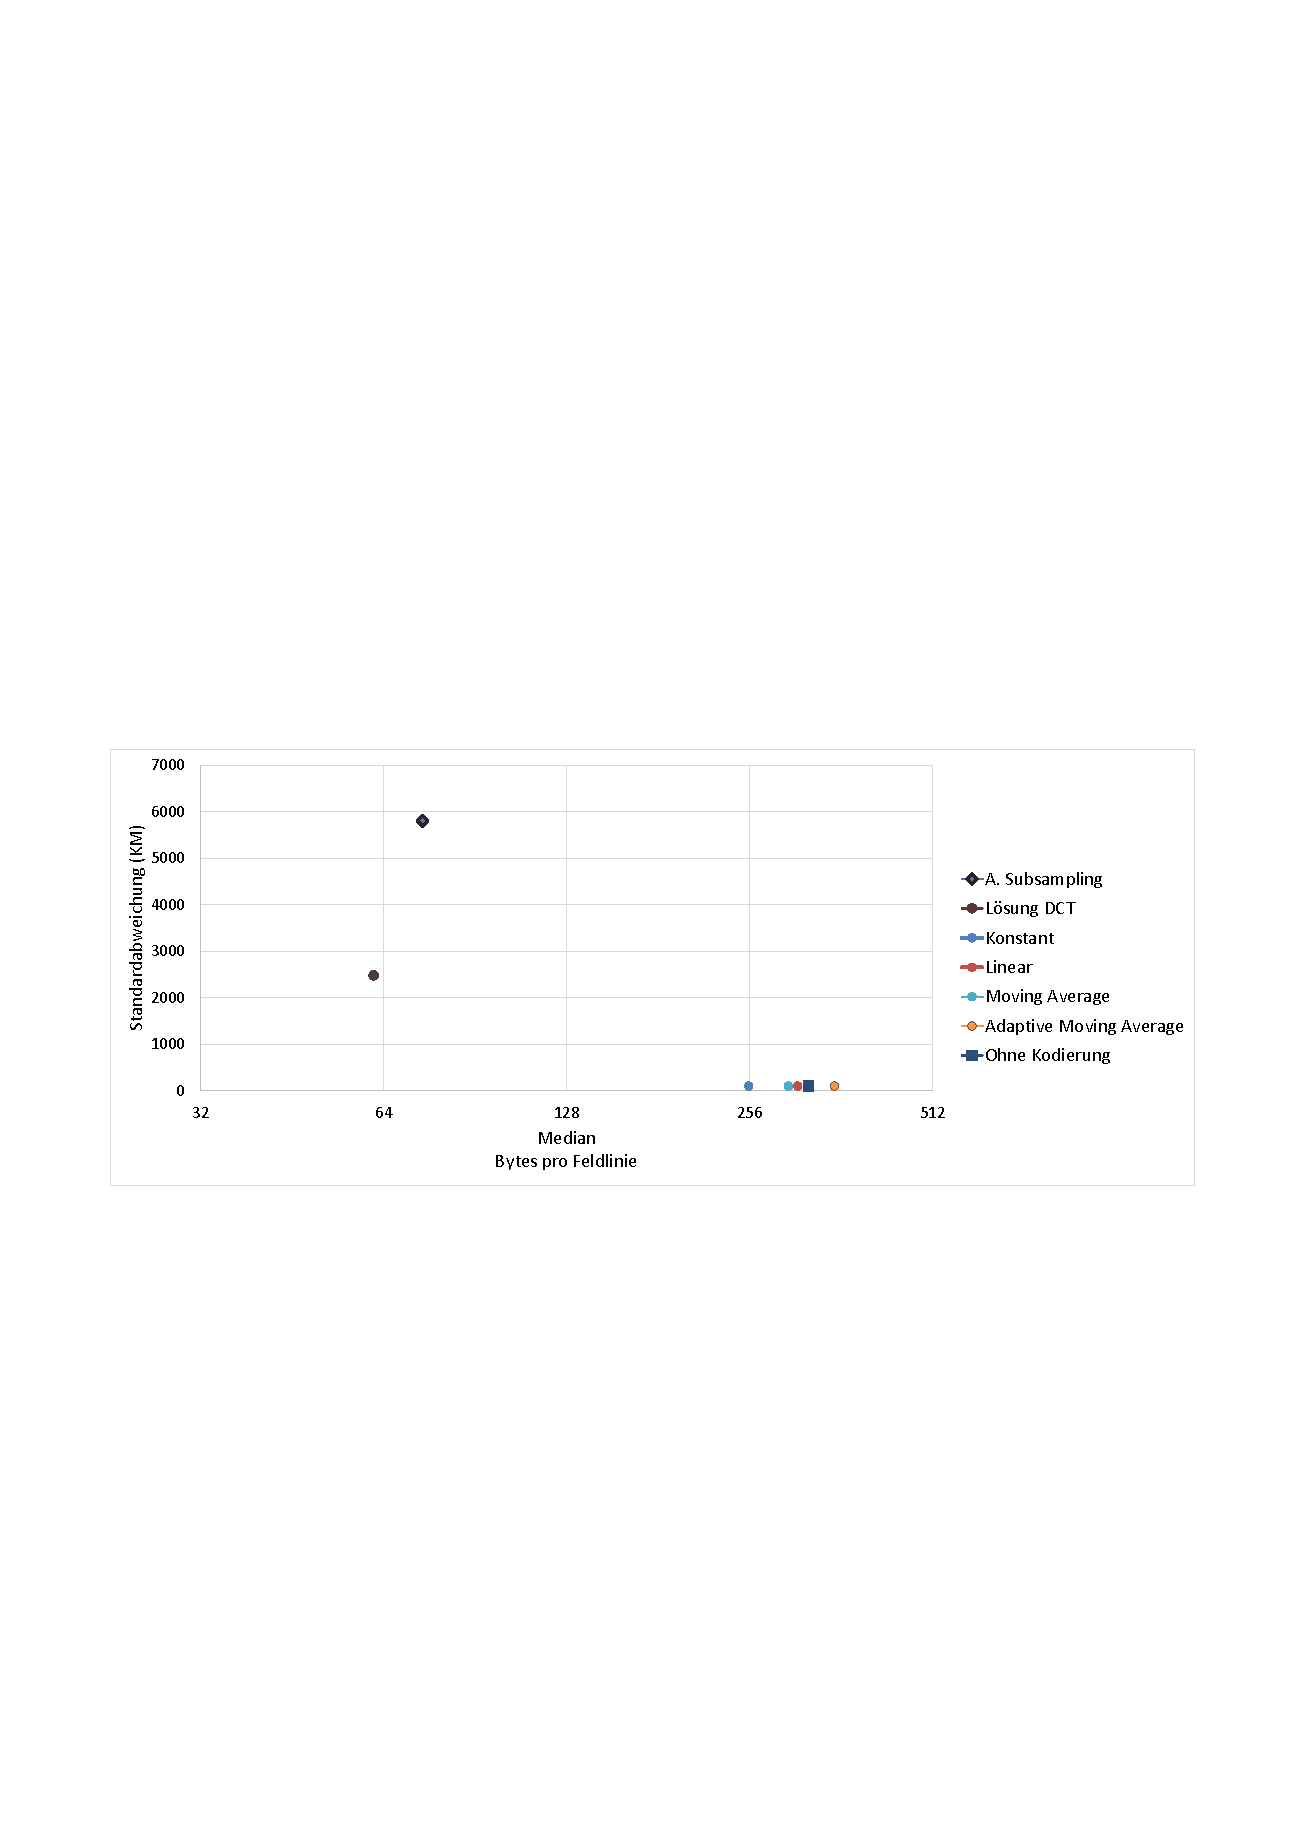
\includegraphics[trim = 1.8cm 11cm 1.8cm 12.5cm, clip=true,width=1\textwidth,keepaspectratio]{./pictures/resultate/loesung2/variante0/resultate.pdf}
	\caption{Kompressionsraten der vier Prediktoren im Vergleich zum Ist-Zustand.}
	\label{resultate:loesung2:simple:resultate}
\end{figure}
Im Diagramm der Abbildung \ref{resultate:loesung2:simple:resultate} sind die Kompressionsraten der jeweiligen Prädiktoren dargestellt. Ein Diagramm mit der PSNR-HVS-M wurde nicht erstellt. Sie ist für alle Prädiktoren gleich und liegt bei 140.7 dB. Unerwartet ist, dass der Konstante Prädiktor mit 255 Bytes pro Feldlinie die höchste Kompressionsrate erreichte, obwohl die Daten nicht zuverlässig vorhergesagt werden. Im Vergleich mit dem Moving Average Prädiktor sind die Fehler der Vorhersagen bis zu 5 Mal grösser, verbrauchen aber 40 Bytes weniger um eine Feldlinie abzuspeichern. Eine Erklärung ist, dass die RAR Kodierung sich wiederholende Muster findet.

Eine mögliche Optimierung ist die adaptive Genauigkeits-Kodierung des DCT Kompressionsverfahrens, beschrieben im Abschnitt \ref{konzept:loesung1:kodierung}. Das Diagramm der Abbildung \ref{resultate:loesung2:simple:resultate_byte} zeigt die Resultate mit der Kodierung. Der Konstante Prädiktor verbraucht mit der adaptiven Genauigkeits-Kodierung mehr Speicherplatz. Die Kompressionsrate der anderen Prädiktoren wird durch die adaptive Genauigkeits-Kodierung deutlich verbessert. Der Lineare Prädiktor erreicht mit 214 Bytes pro Feldlinie und einer Kompressionsrate von 4 das beste Resultat. Es bestätigt die Vermutung, dass der Konstante Prädiktor keine zuverlässige Vorhersage erreichte und die Kompressionsrate auf die RAR Kodierung zurückzuführen ist.

\begin{figure}[!htbp]
	\center
	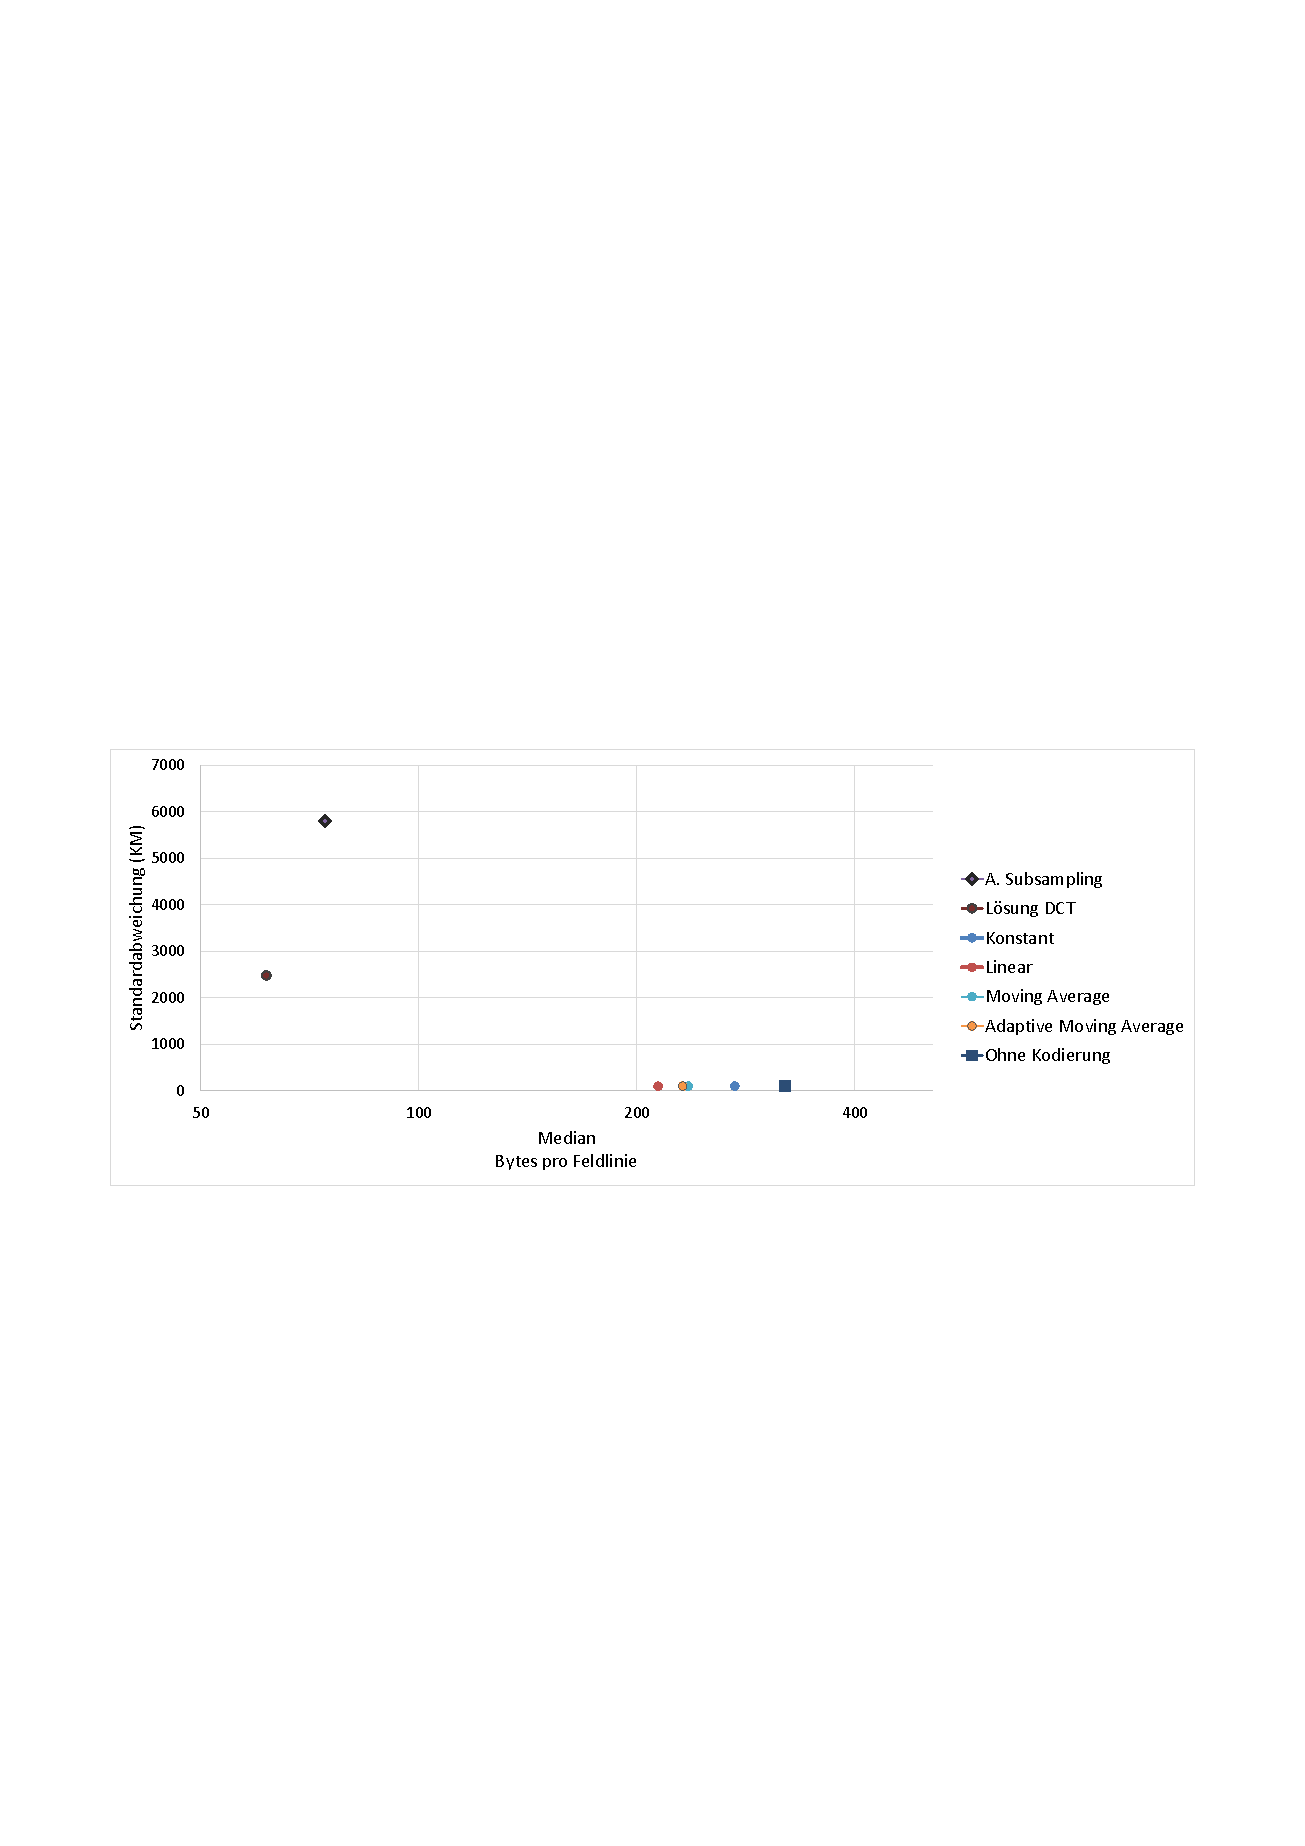
\includegraphics[trim = 1.8cm 11cm 1.8cm 12.5cm, clip=true,width=1\textwidth,keepaspectratio]{./pictures/resultate/loesung2/variante0/resultate_byte.pdf}
	\caption{Kompressionsraten der Prediktoren mit adaptiver Genauigkeits-Kodierung.}
	\label{resultate:loesung2:simple:resultate_byte}
\end{figure}

\subsubsection{Variante: Adaptives Subsampling} \label{resultate:loesung2:adaptive}
Um mit der Kompressionsrate der Prädiktiven Kodierung in dieselbe Grössenordnung zu gelangen wie die Kompressionen des Adaptives Subsampling oder der DCT müssen mehr Informationen gelöscht werden. Deshalb wird das Adaptive Subsampling eingesetzt, es werden andere Parameter verwendet und im Schnitt 50\% mehr Daten übertragen als in der Kompression mittels Adaptivem Subsampling.

\begin{figure}[!htbp]
	\center
	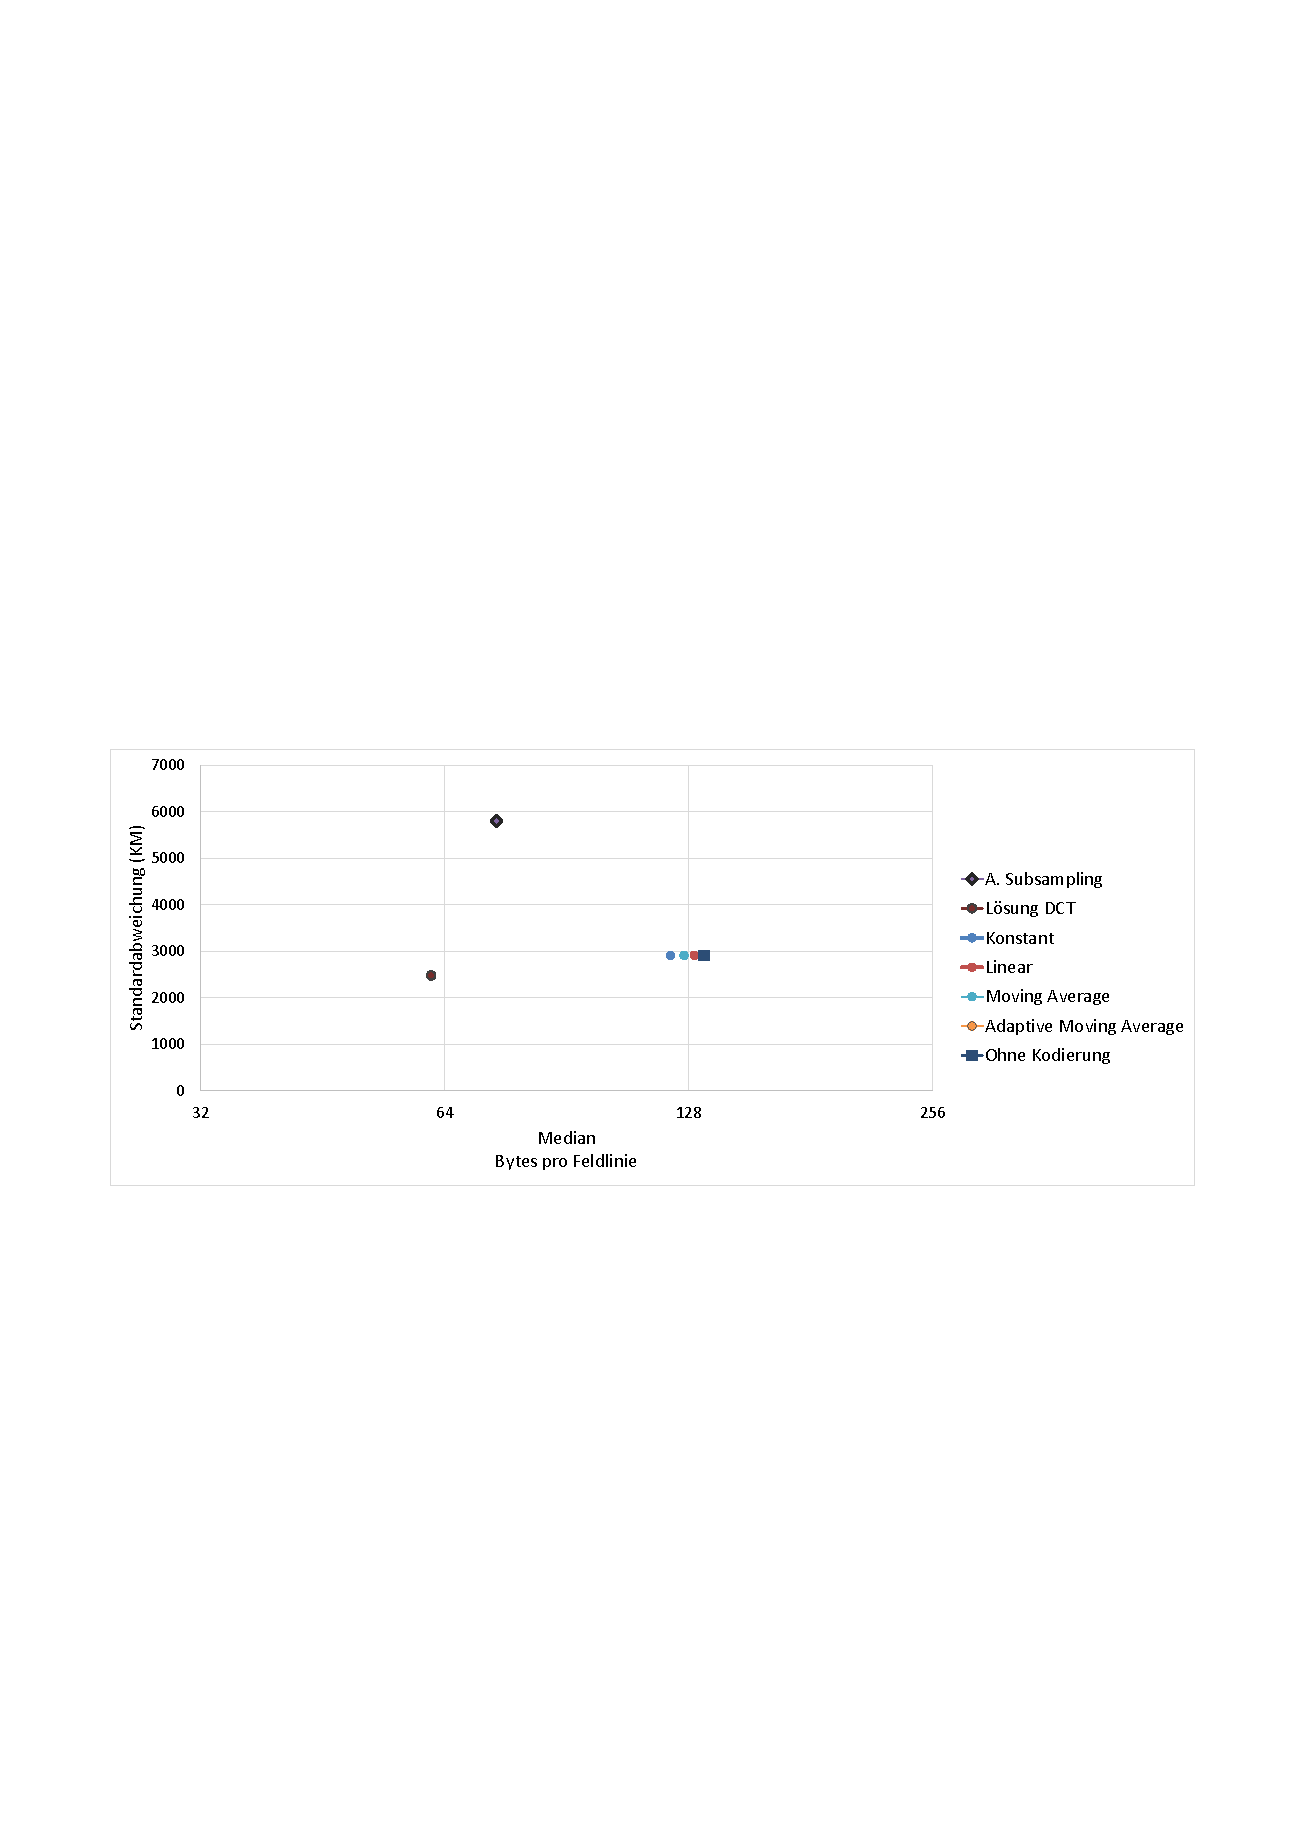
\includegraphics[trim = 1.8cm 11cm 1.8cm 12.5cm, clip=true,
width=1\textwidth,keepaspectratio]{./pictures/resultate/loesung2/variante1/resultate_euler.pdf}
	\caption{Kompressionsraten der Prediktiven Kodierungen mit dem Adaptiven Subsampling.}
	\label{resultate:loesung2:adaptive:euler}
\end{figure}
Das Diagramm der Abbildung \ref{resultate:loesung2:adaptive:euler} zeigt die Kompressionsraten. Die Resultate liegen dicht beieinander und der Abstand zwischen Kodierung und der Kompression, welche ohne Kodierung erreicht wird, wurde drastisch vermindert. Die Kodierungen erreichen eine PSNR-HVS-M von 139,2. Das Angle Subsampling verändert die Eigenschaften der Daten. Die Diagramme der Abbildung \ref{resultate:loesung2:adaptive:channel} zeigen die Veränderung: Monotone Steigungen sind nach dem Subsampling nicht mehr vorhanden. Die einfachen Prädiktoren können die Daten nicht zuverlässig vorhersagen.

\begin{figure}[!htbp]
	\center
	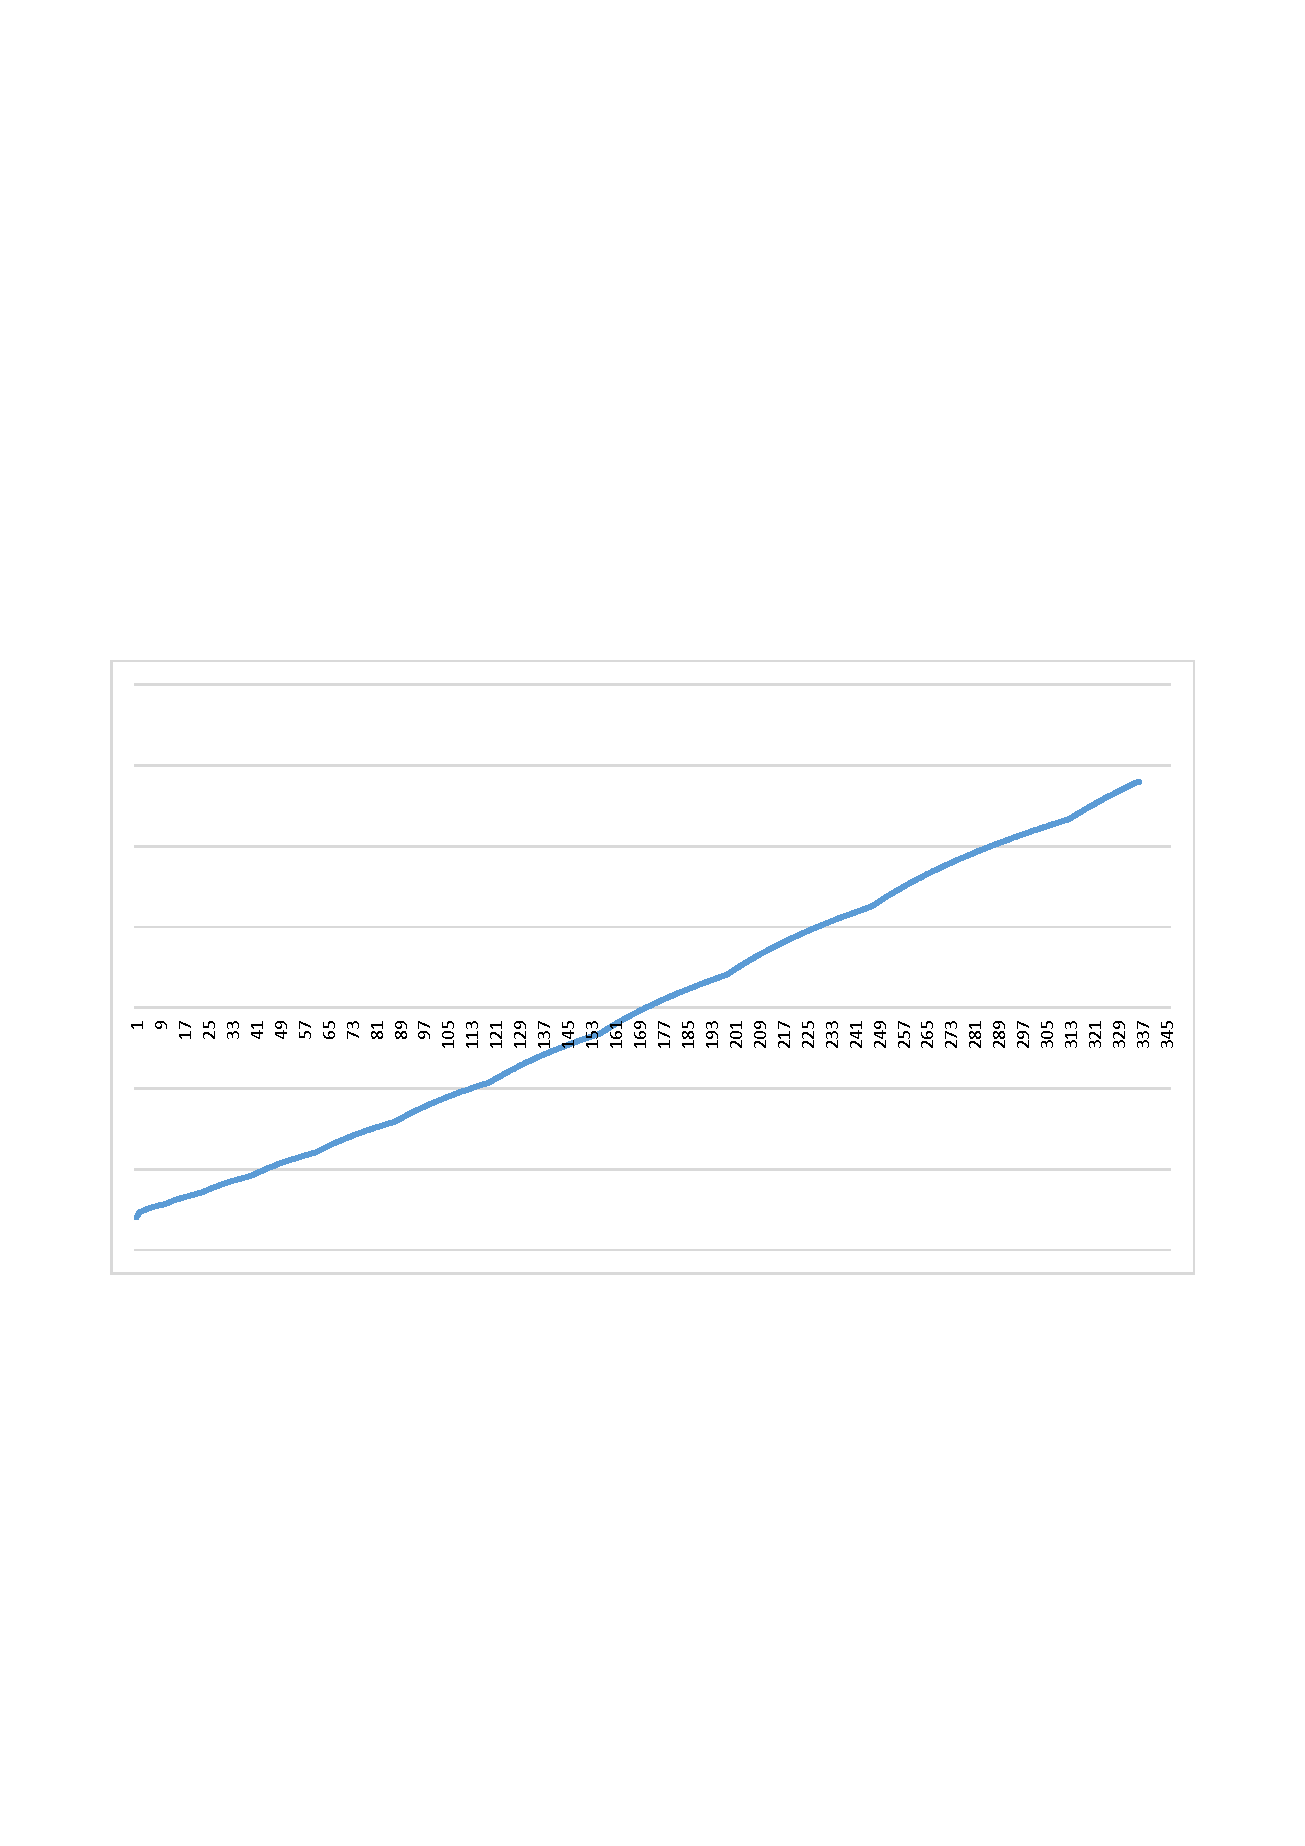
\includegraphics[trim = 1.8cm 9.5cm 1.8cm 11cm, clip=true,
width=0.49\textwidth,height=5cm,keepaspectratio]{./pictures/resultate/loesung2/variante1/channel_euler.pdf}
	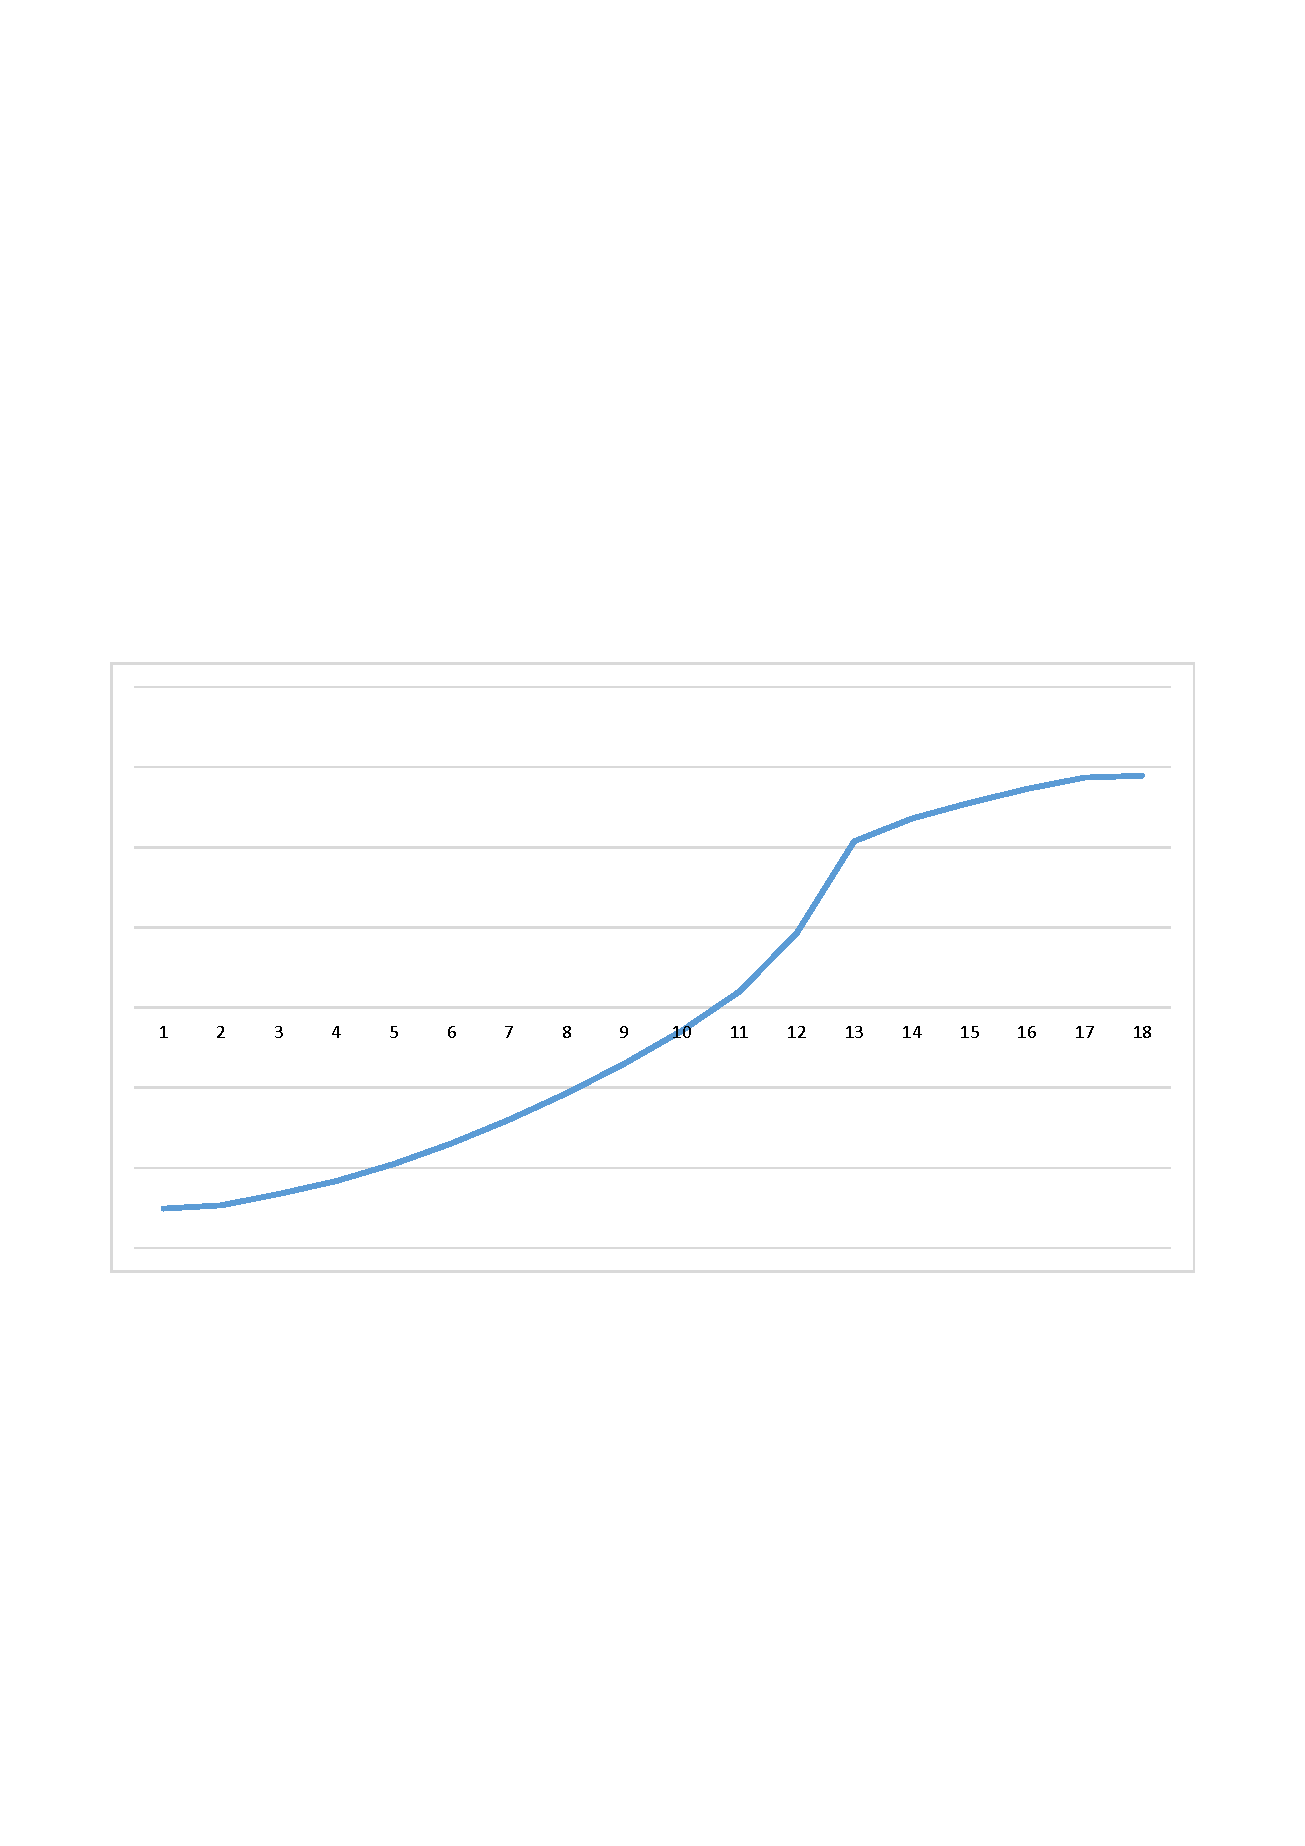
\includegraphics[trim = 1.8cm 9.5cm 1.8cm 11cm, clip=true,
width=0.49\textwidth,height=5cm,keepaspectratio]{./pictures/resultate/loesung2/variante1/channel_angle.pdf}
	\caption{Änderung der Eigenschaften der Daten durch das Adaptive Subsampling. Links der Kanal einer Feldlinie vor, rechts der Kanal nach dem Adaptiven Subsampling.}
	\label{resultate:loesung2:adaptive:channel}
\end{figure}

\subsubsection{Rekursive Lineare Kodierung} \label{resultate:loesung2:wavelet}
Die Rekursive Lineare Kodierung ist in der Lage für nicht-stetige Kanäle eine sinnvolle Vorhersage zu berechnen. Das Verfahren ist im Abschnitt \ref{konzept:prediktiv} genauer erläutert. Die Punkte werden ins sphärische Koordinatensystem überführt. In diesem Koordinatensystem sind 16 Bit Genauigkeit pro Koordinatenachse ausreichend und die PCA muss nicht berechnet werden. Im Schnitt können dadurch 30 Bytes pro Feldlinie eingespart werden. Zusätzlich werden die Vorhersagefehler quantisiert.

\begin{figure}[!htbp]
	\center
	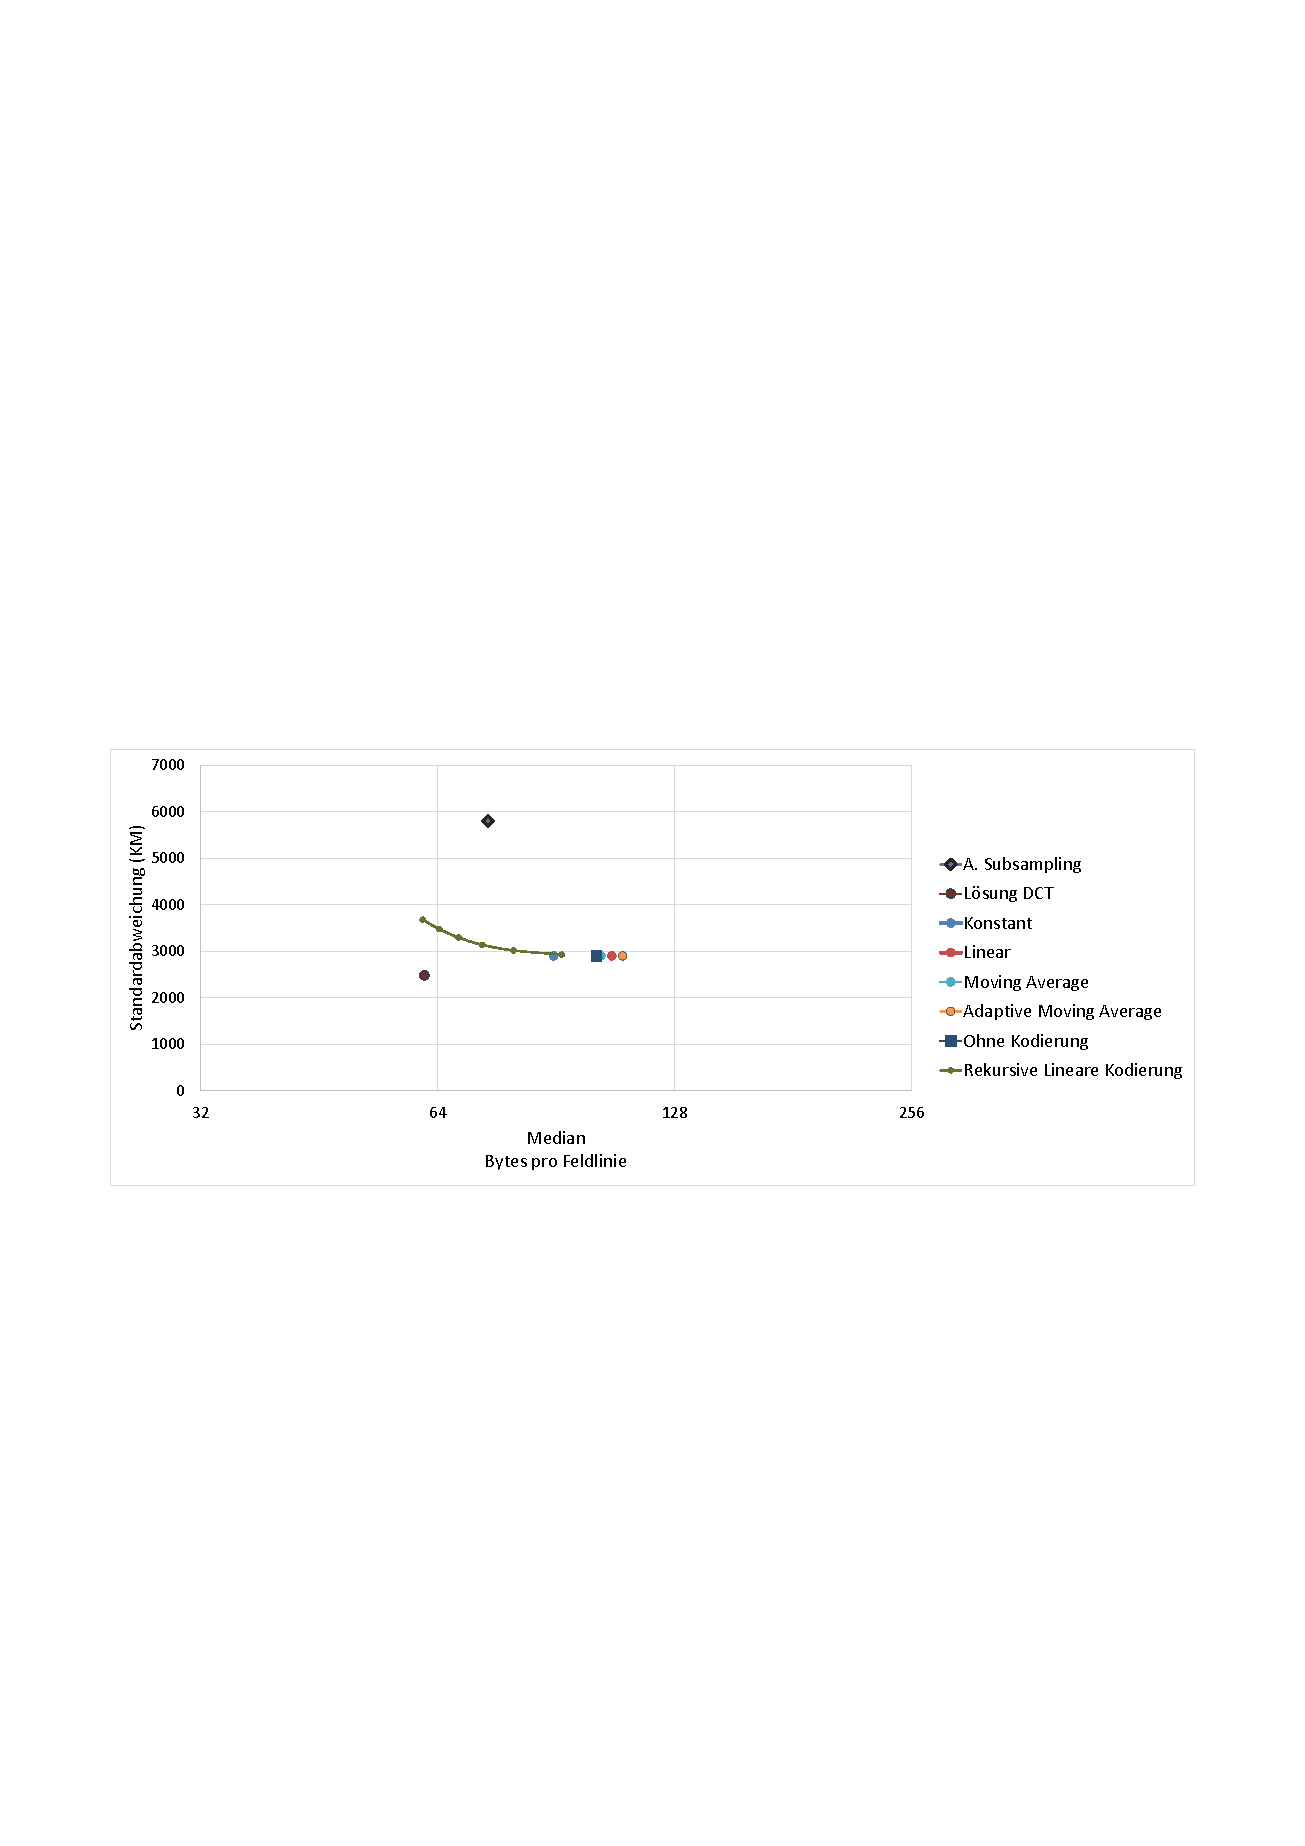
\includegraphics[trim = 1.8cm 11cm 1.8cm 12.6cm, clip=true,width=1\textwidth,keepaspectratio]{./pictures/resultate/loesung2/variante2/resultate_median.pdf}
	
	\caption{Kompressionsraten der Rekursiven Linearen Kodierung mit dem Adaptiven Subsampling.}
	\label{resultate:loesung2:adaptive:median}
\end{figure}
\begin{figure}[!htbp]
	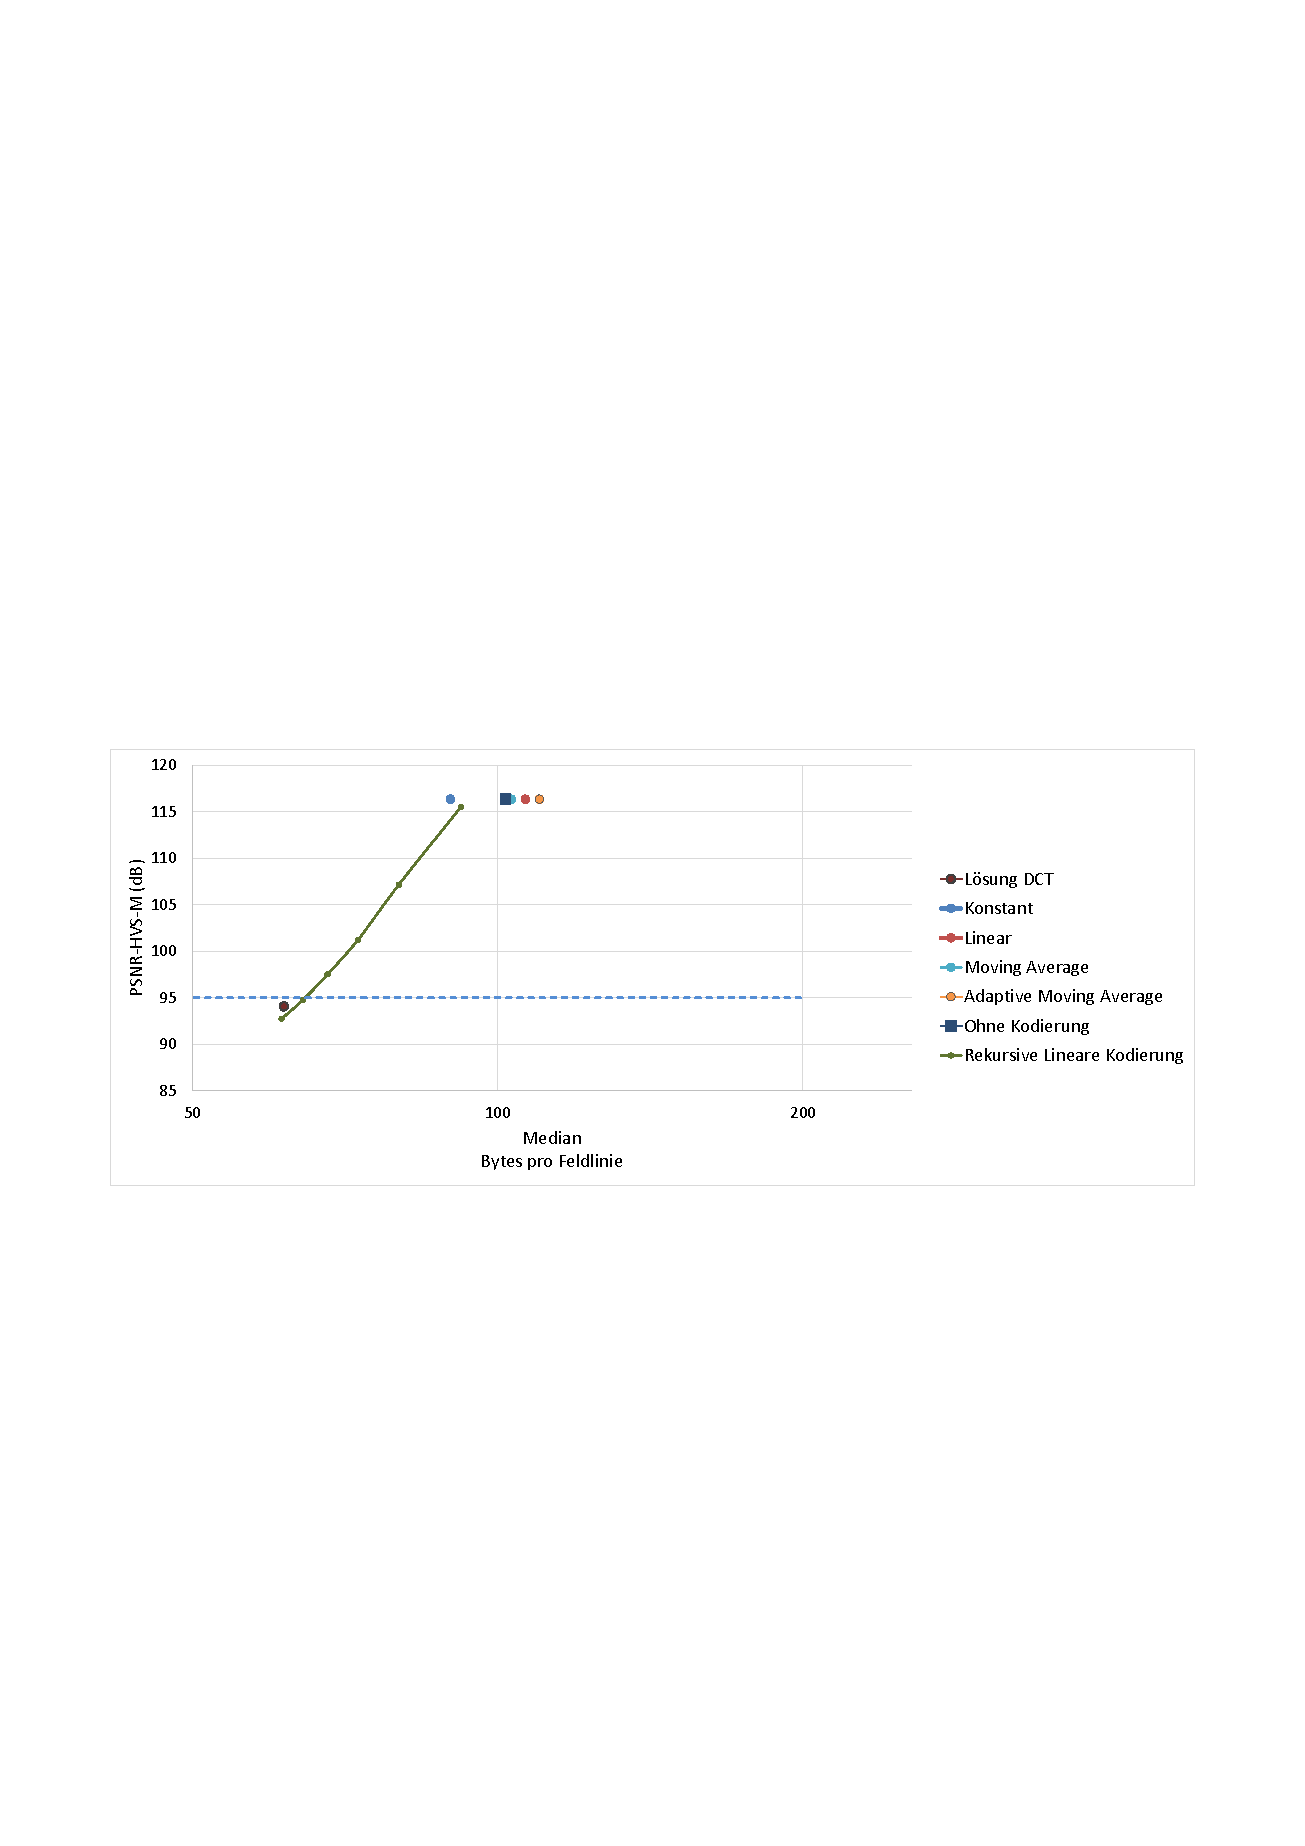
\includegraphics[trim = 1.8cm 11cm 1.8cm 12.6cm, clip=true,width=1\textwidth,keepaspectratio]{./pictures/resultate/loesung2/variante2/resultate_psnr.pdf}
	
	\caption{Kompressionsraten der Rekursiven Linearen Kodierung mit dem Adaptiven Subsampling.}
	\label{resultate:loesung2:adaptive:median_psnr}
\end{figure}
Das Diagramm der Abbildung \ref{resultate:loesung2:adaptive:median} zeigt die Standardabweichung der Rekursiven Linearen Kodierung zu unterschiedlichen Quantisierungen. Das Diagramm der Abbildung \ref{resultate:loesung2:adaptive:median_psnr} zeigt die PSNR-HVS-M Werte der Variante. Die Resultate der einfachen Prädiktoren wurden ebenfalls ohne PCA im sphärischen Koordinatensystem gemessen. Die Rekursive Lineare Kodierung kann eine bessere Kompressionsrate erreichen als die Kompression mit Adaptiven Subsampling. Bei Datenmenge von 64 Bytes pro Feldlinie erreicht diese Variante eine tiefere Standardabweichung als das Adaptive Subsampling zu einem PSNR-HVS-M Wert von 94.7. Diese Variante besitzt ausserdem weniger ausgeprägte Artefakte als das DCT Verfahren, weist aber eine höhere Standardabweichung auf. Die Variante erreicht eine Kompressionsrate von 13.4 und fällt somit zwischen den Kompressionen mittels DCT und Adaptives Subsampling.

Die Artefakte der Dekompression äussern sich meist als Verschiebungen einzelner Punkte. Im Extremfall können ringing-ähnliche Artefakte entstehen, die in der Abbildung \ref{resultate:loesung2:adaptive:median:artefakte} dargestellt sind. Der Grund für die Artefaktbildung liegt in der Rekursion: Wenn der Vorhersagefehler des ersten Wertes (siehe Diagramm der Abbildung \ref{konzept:loesung2:algorithm:step1}) quantisiert wird, beeinflusst der Quantisierungsfehler den gesamten Kanal. Die Werte, welches als letztes kodiert werden, erfahren die grösste Verschiebung bei der Dekompression. Diese Variante verwendet einen konstanten Faktor für die Quantisierung. Die Lösung ist eine angepasste Quantisierung, welche die ersten Vorhersagefehler der ersten Rekursionsstufe mit höherer Genauigkeit abspeichert.

\begin{figure}[!htbp]
	\center
		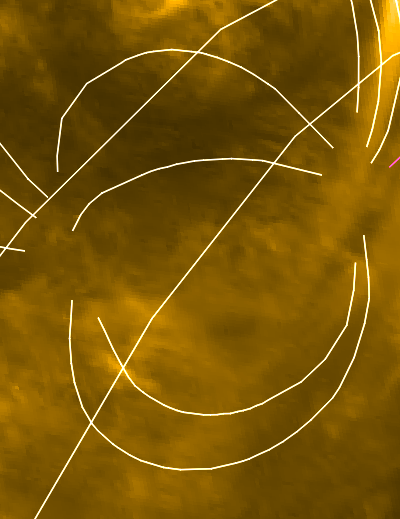
\includegraphics[width=0.49\textwidth,height=5cm,keepaspectratio]{./pictures/resultate/loesung2/variante3/no_artifacts.png}
	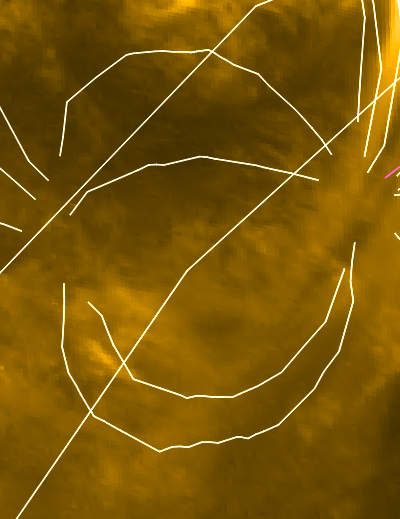
\includegraphics[width=0.49\textwidth,height=5cm,keepaspectratio]{./pictures/resultate/loesung2/variante3/artifacts_8.png}
	\caption{Artefakte der Rekursiven Linearen Kodierung. Links sind die originalen Feldlinien.}
	\label{resultate:loesung2:adaptive:median:artefakte}
\end{figure}

\subsubsection{Rekursive Lineare Kodierung mit angepasster Quantisierung}
Um die Artefakte der Dekompression zu dämpfen, werden die Vorhersagefehler der Rekursionsstufe angepasst quantisiert. Die ersten Rekursionsstufen werden mit höherer Genauigkeit abgelegt.

\begin{figure}[!htbp]
	\center
	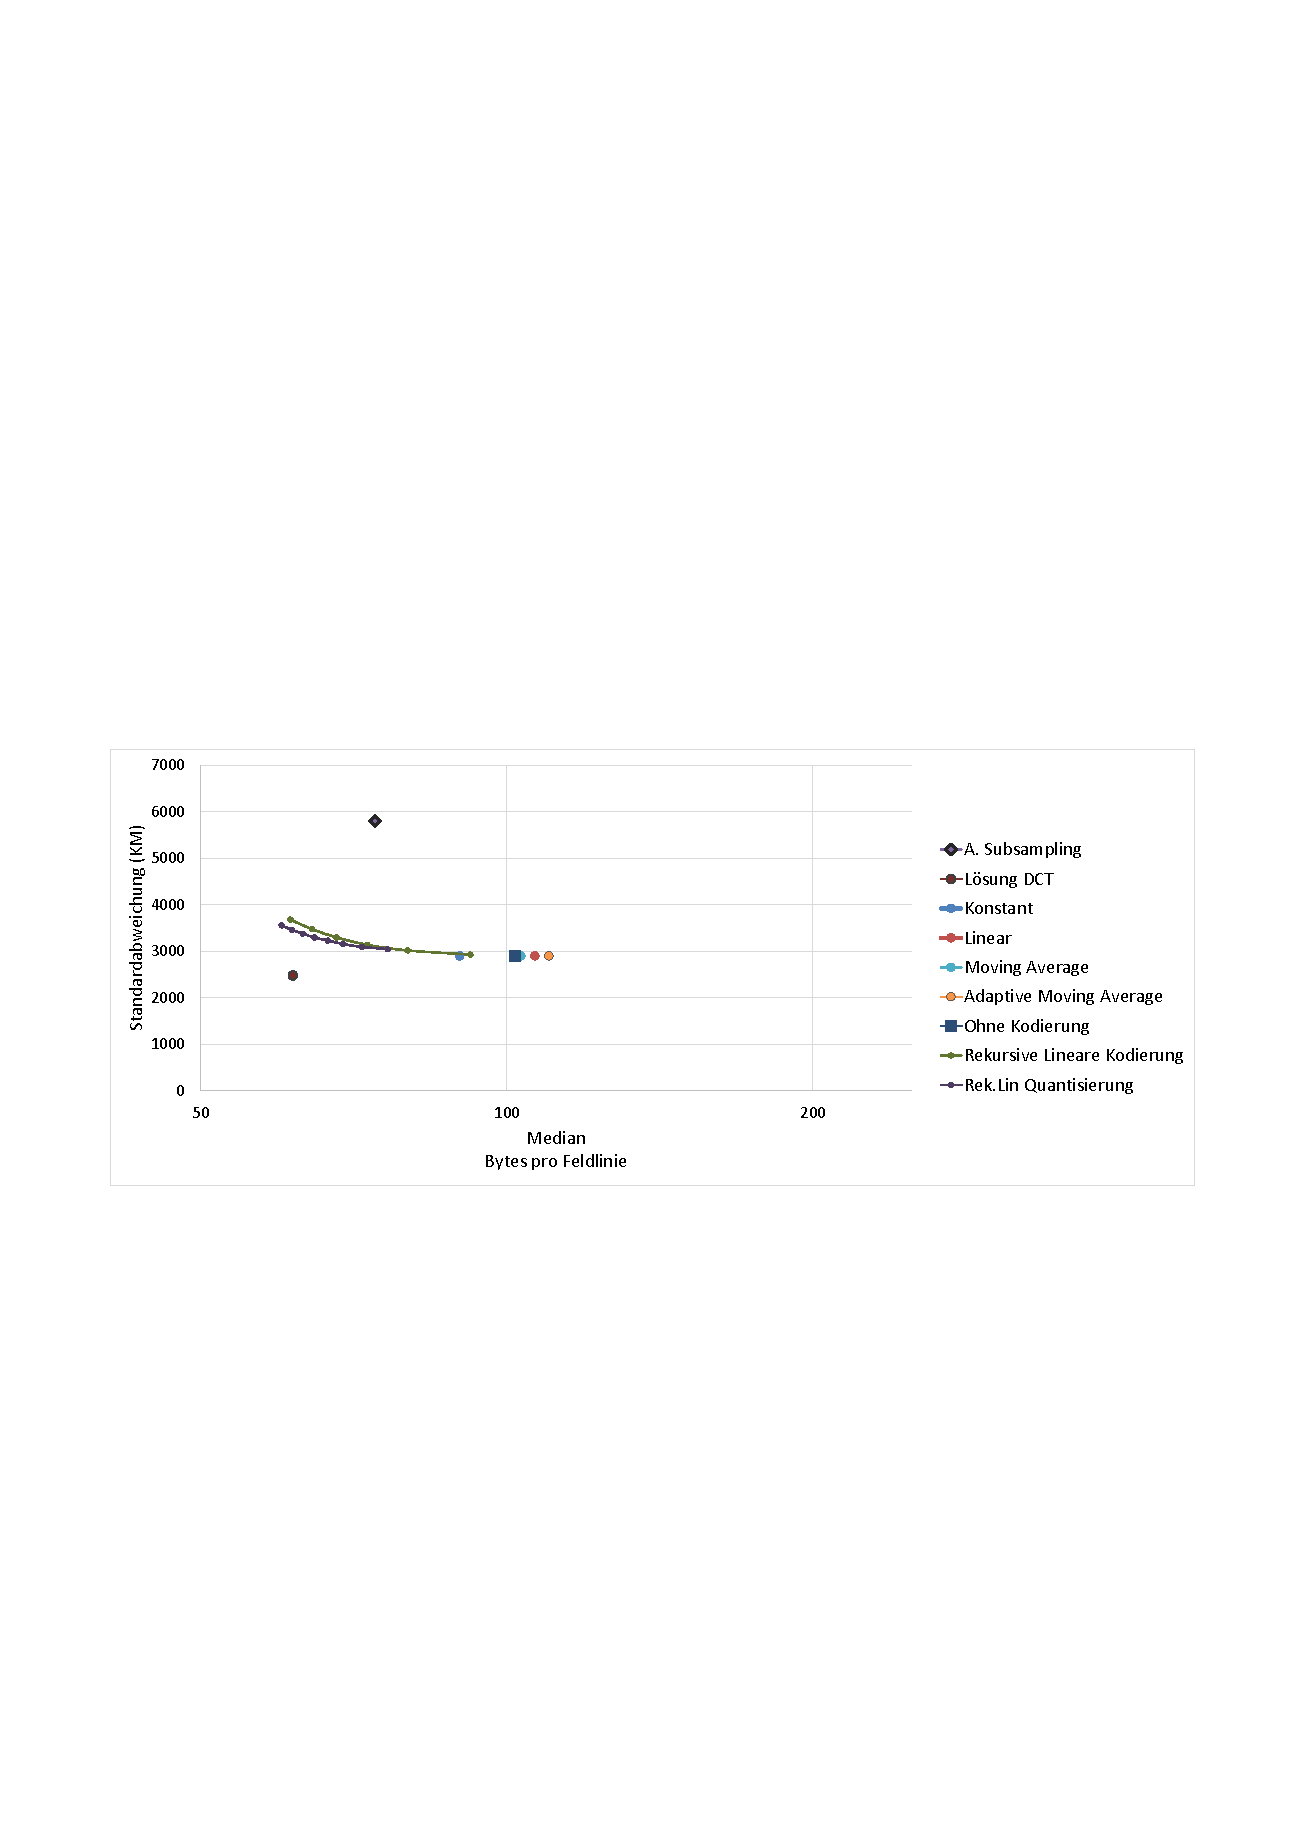
\includegraphics[trim = 1.8cm 11cm 1.8cm 12.5cm, clip=true,width=1\textwidth,keepaspectratio]{./pictures/resultate/loesung2/variante3/resultate.pdf}
		\caption{Standardabweichung der Rekursiven Linearen Kodierung mit angepasster Quantisierung.}
		\label{resultate:loesung2:adaptive:median:quant}
\end{figure}
\begin{figure}[!htbp]
\center
	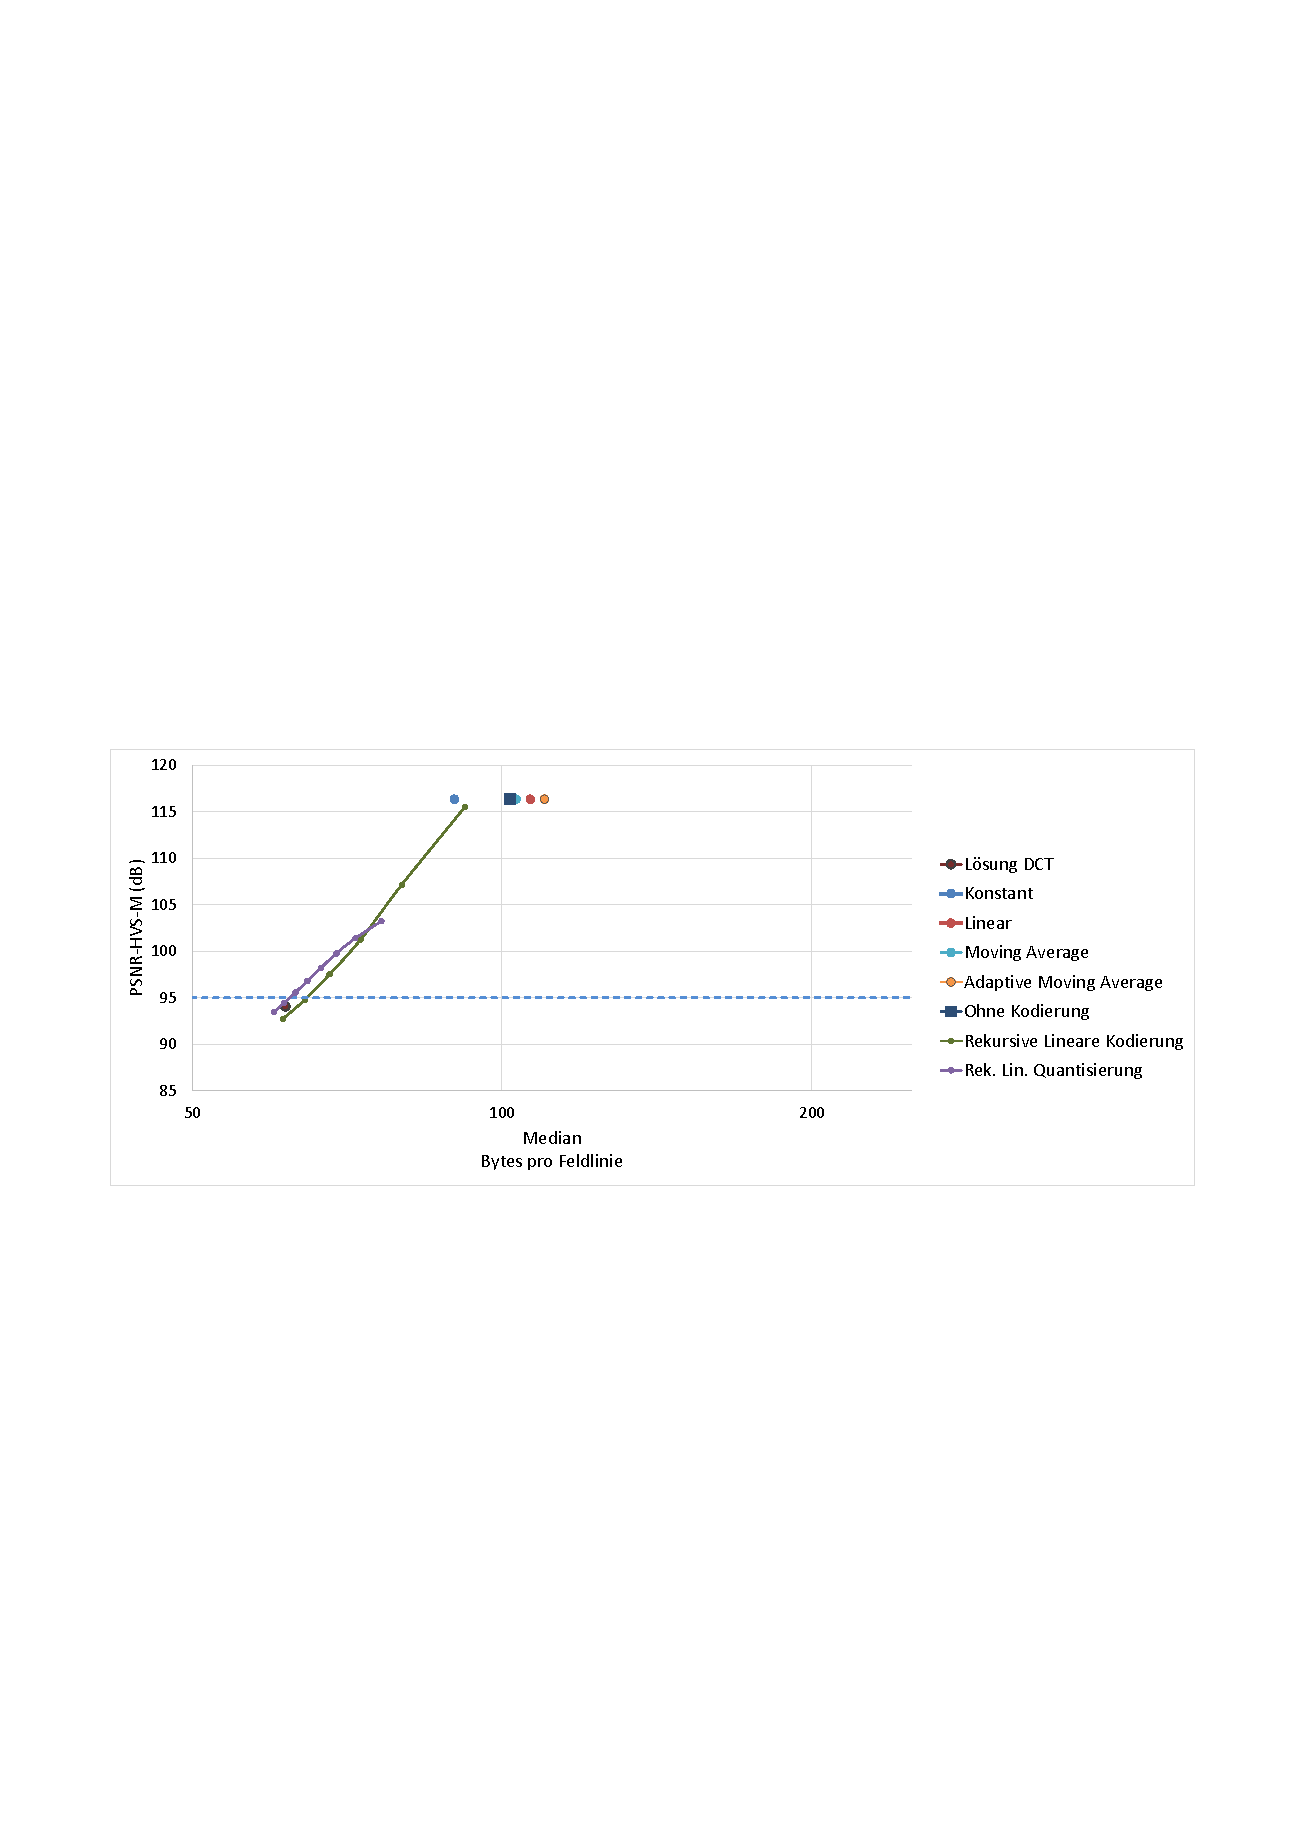
\includegraphics[trim = 1.8cm 11cm 1.8cm 12.5cm, clip=true,width=1\textwidth,keepaspectratio]{./pictures/resultate/loesung2/variante3/resultate_psnr.pdf}
	\caption{PSNR-HVS-M der Rekursiven Linearen Kodierung mit angepasster Quantisierung.}
	\label{resultate:loesung2:adaptive:median:quant_psnr}
\end{figure}
Die angepasste Quantisierung bringt eine Verbesserung in der Standardabweichung mit sich. Die Diagramme der Abbildungen \ref{resultate:loesung2:adaptive:median:quant} und \ref{resultate:loesung2:adaptive:median:quant_psnr} visualisieren die Standardabweichung und PSNR-HVS-M zur jeweiligen Kompression. Mit der angepassten Quantisierung kann diese Variante eine ähnliche Kompressionsrate zu höherer PSNR-HVS-M erreichen, als das Verfahren mittels DCT. Mit einer PSNR-HVS-M von 95.5 verbraucht diese Variante 63 Bytes pro Feldlinie, was zu einer Kompressionsrate von 13.6 führt.

Die Artefakte haben sich im Vergleich zur vorhergehenden Variante verbessert: Die Abbildung \ref{resultate:loesung2:adaptive:median_extra:artefakte} zeigt die Artefaktbildung dieser Variante. Die ringing-ähnlichen Artefakte sind verschwunden. In dieser Variante äussern sich Kompressionsartefakte als Verschiebung einzelner Punkte. Bei hoher Dichte der Feldlinien werden die Verschiebungen sichtbar, da sie sich je nach Blickwinkel häufiger kreuzen und eine unästhetische Visualisierung ergeben. Eine leichte Glättung der Feldlinien versteckt die Artefakte und gestaltet eine ästhetische Visualisierung.

\begin{figure}[!htbp]
	\center
		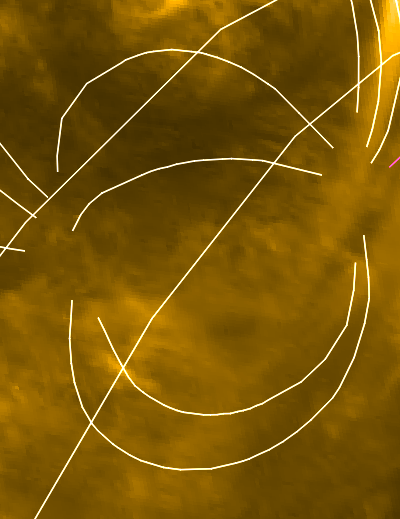
\includegraphics[width=0.49\textwidth,height=5cm,keepaspectratio]{./pictures/resultate/loesung2/variante3/no_artifacts.png}
	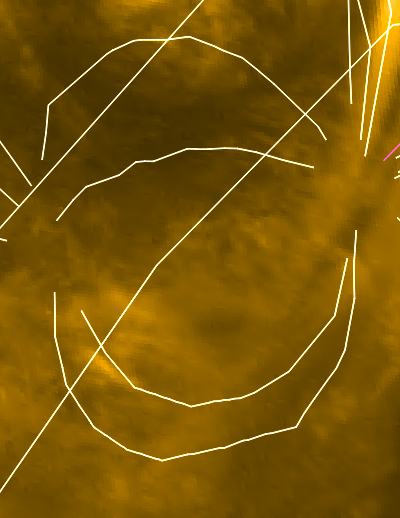
\includegraphics[width=0.49\textwidth,height=5cm,keepaspectratio]{./pictures/resultate/loesung2/variante3/artifacts_extra.png}
	\caption{Artefakte der Rekursiven Linearen Kodierung mit angepasster Quantisierung.Links sind die originalen Feldlinien.}
	\label{resultate:loesung2:adaptive:median_extra:artefakte}
\end{figure}

Das Caching von 1000 Simulationen und die Übertragungszeit fallen zwischen die anderen Kompressionsverfahren mit 72 Megabyte an Arbeitsspeicher beziehungsweise 118 Sekunden Übertragungszeit. Zum Vergleich: Die DCT Variante verbraucht unter denselben Bedingungen 70 und das Adaptive Subsampling 85 Megabyte an Arbeitsspeicher. Bei einer Internetverbindung von 5 Megabit ist bei diesem Verfahren mit einer Übertragungsrate von 8 Simulationen in der Sekunde zu rechnen. Die Laufzeit der Dekompression liegt mit 30.6 Millisekunden ebenfalls zwischen den Kompressionsverfahren Adaptives Subsampling und DCT (siehe Abschnitt \ref{anhang:performance}). Mit dieser Laufzeit kann ein Thread durchschnittlich 32 Simulationen pro Sekunde dekomprimieren.